\section{Look Ahead}
\subsection{Theory of Operation}

The look ahead node is responsible for obstacle detection. The node
subscribes to lidar data and uses trigonometric functions to check for
obstacles within a bounded box.  The box's dimensions are currently 1m
in front of the robot and .25m on either side. 

The node constantly publishes to the obstacles topic using a custom
message type of ``Obstacle''.  The Obstacle message and the
subscribers of the obstacle topic are described in Custom Message
Specifications section.

In order to perform its job the Look Ahead node subscribes to the
lidar data published with message type sensor\_msgs/laserscan. This message
includes information about each laser ping's distance and intensity as
well as information about the laser range finder device itself.  In
our case, the lidar is set to do 181 pings on every sweep with spacing
of 1 degree per ping.  This works out to a sweep from -90$^\circ$ to
90$^\circ$ in the robots base coordinate frame.

When an obstacle is detected in the box the obstacles boolean in the
Obstalce message type is set to true. The algorithm also calculates
the closest of the obstacle pings and puts that number in the distance field
of the Obstacle message type. When no obstacles are detected obstacles
is set to false and distance is set to 0.0.

\subsubsection{Implementation Decisions}

To account for the possibility of more pings per sweep or sweeps of
smaller degrees we have constants that are defined globally at the top
of the file.  This gives us a single place to change fundamental
parameters of the program.  We could potentially move these into a
configuration file to prevent the need to recompile when new settings
are desired.

\subsubsection{Bounding Box Algorithm}
To determine if a ping is within the box dimensions the trigonometric
functions are used to determine the bounds of the box.  For each ping
a maximum distance is computed.  If the ping distance is larger than this
value then it is ignored. If the ping distance is less it is
considered an obstacle.  The minimum of all pings within the distance
thresholds is returned as the distance.

\FloatBarrier
\begin{figure}[h]
  \centering
  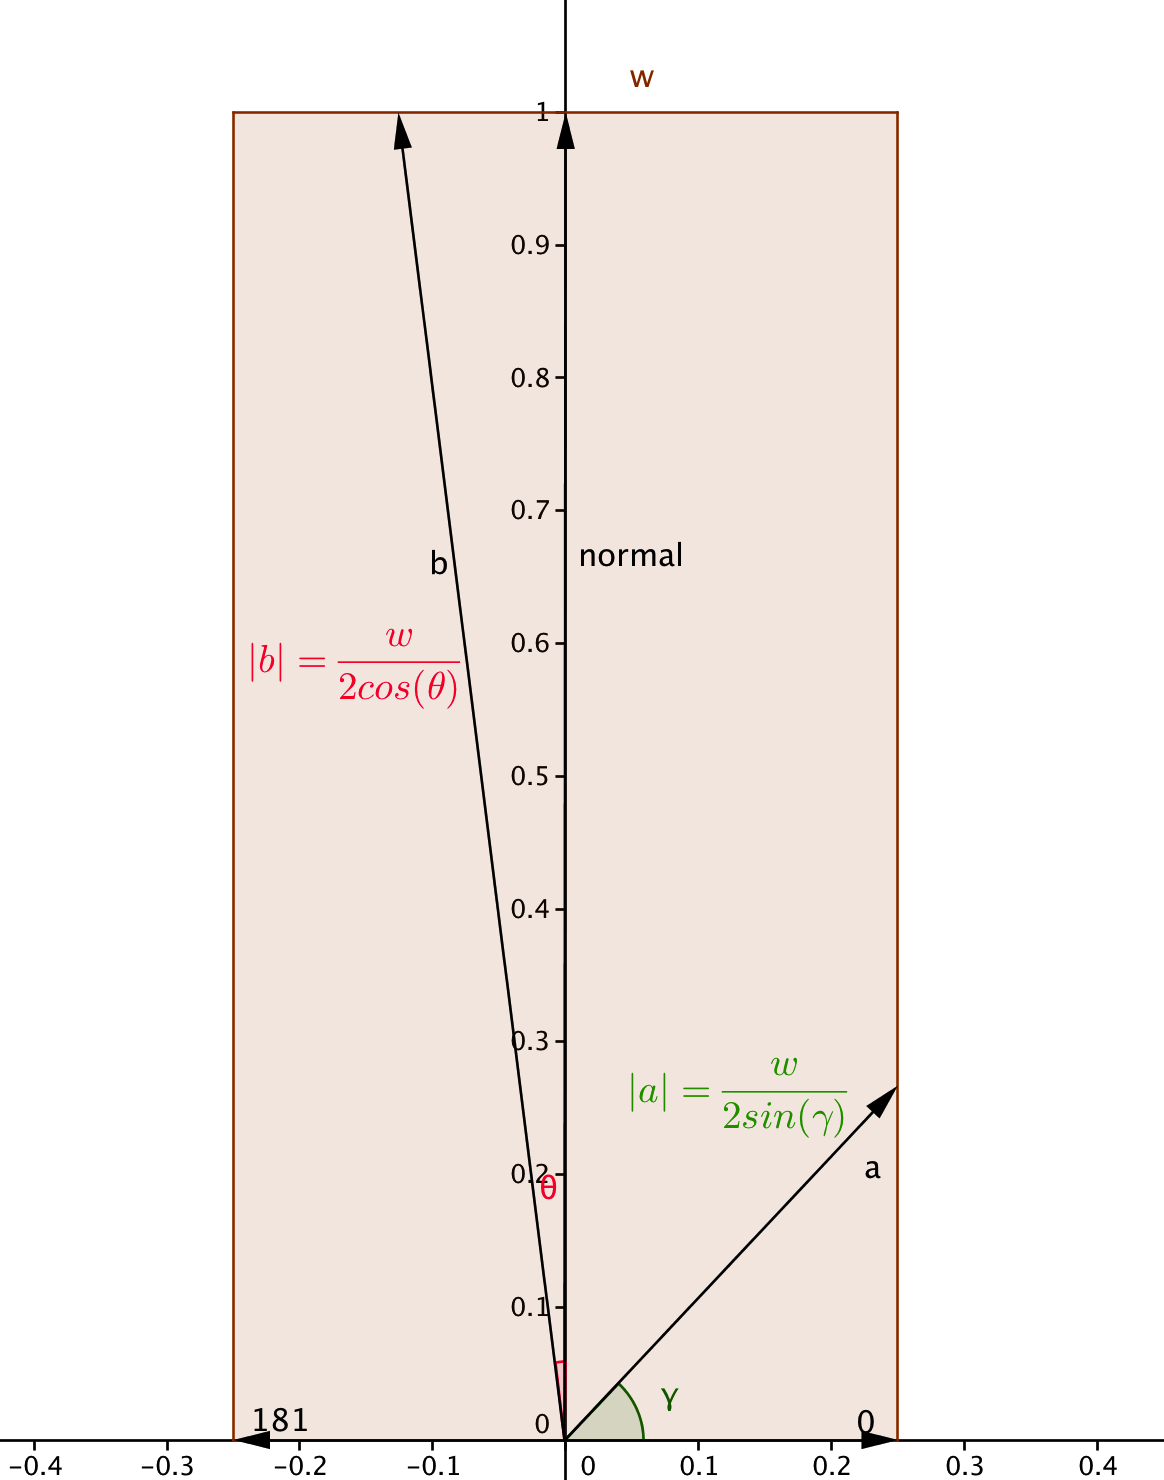
\includegraphics[height=4.5in]{Look_Ahead_Bounding_Box.png}
  \caption{Calculations for laser ping distances}
\end{figure}
\FloatBarrier

In this figure a laser ping from each of the two region types is shown
along with the function used to calculate the maximum distance.

\FloatBarrier
\begin{figure}[h]
  \centering
  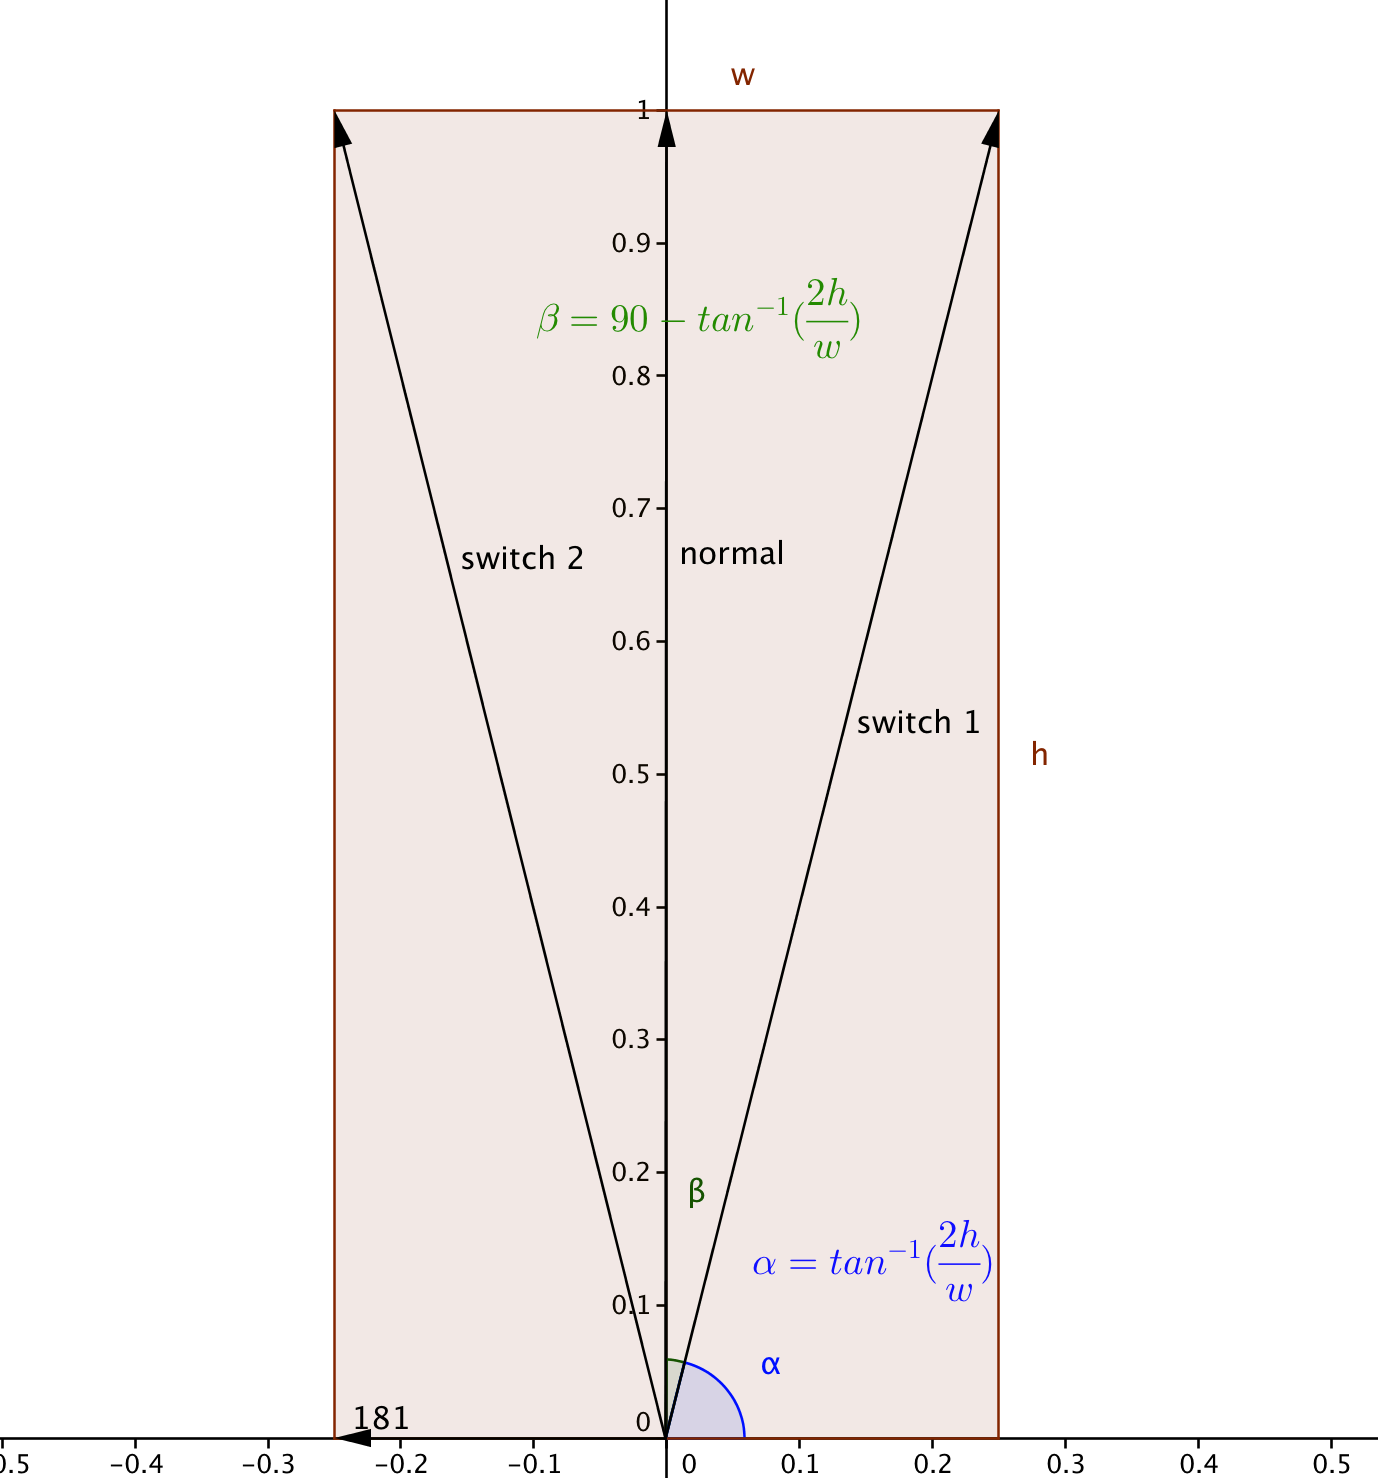
\includegraphics[height=4.5in]{look_ahead_bounding_box_transitions.png}
  \caption{Calculations for the transition angles}
\end{figure}
\FloatBarrier

This figure shows what how the transition angles are calculated.
After the ping corresponding to one of the transition angles is surpassed,
the calculations for the next set of pings switches between the two
equations shown in figure 3.

\subsection{Observations}

\subsubsection{Lidar Problems}
Because of the LIDAR's limited angular range, it is not very useful
for obstacle detection during turning.  The positioning of the LIDAR
unit prevents it from seeing obstacles to its side or behind it. While
we have the ability to decide if a turn is safe before we reaching the
starting point, we don't
have the ability to detect a new obstacle after the turn has started.

In addition we need to verify that the LIDAR gives consistent and
accurate data during turns.  The LIDAR method uses a rotating mirror
to send out and detect laser pings.\cite{deyle_sick_2008}
Theoretically the added rotation of the robot could ``smear'' the
LIDAR data.  Because we haven't used it during turns we have not
confirmed whether this is the case, but as we add the capabilities for
arcs this potential effect will become more important.

Another peculiarity of the LIDAR is the minimum range.  After an
object gets too close it disappears from the LIDAR.  This is most
likely because the circuitry of the LIDAR cannot detect the return
pulses fast enough to caclulate the data and so it filters them out.
Luckily it appears as if the minimum range is quite close. We found
the cutoff range to be around 0.1 m.

This range is not a problem from the robot's perspective because the
robot should never try to get close enough to object for this to
become an issue.  However, the opposite may not always be true. If the
robot stops for an approaching humand the human walks right up to the
robot without knowing the LIDAR limitations the robot may think the
human has disappeared and continue on its path.

The only potential solution we can see to this is to implement a
detection algorithm that examines where objects disappear, if the
object disappears by the robot's minimum range the robot can assume
the object is still there.  However, if the person leaves the range
while staying within the minimum range, the robot will think the human
is still there and wait forever. Obviously this is not ideal, however
other sensors like the Kinect camera will help us avoid this small, but potentially dangerous problem.


\subsection{Unimplemented Functions}
Because of several code changes there are desirable features of look ahead that we planned on implementing, but did
not have enough time to focus on.


\subsubsection{Obstacle detection on arcs and spins}
 \begin{enumerate}
   \item We considered fattening LIDAR pings and ensuring that fattened LIDAR pings did not pass through the enlarged pings
 
   \item Another option was to use the bounding box algorithim on a linearized arc path segment.
   \item  The idea became unecessary because the steering node steers from map point to map point instead of by path segments.
  \end{enumerate}






